This section includes a class diagram which is representative of the relevant features of the system-to-be, followed by the Alloy code that describes and checks the consistency of the model provided in this document, as well as an example of the model-compliant world generated by the Alloy tool.

\begin{figure}[H]
\begin{center}
		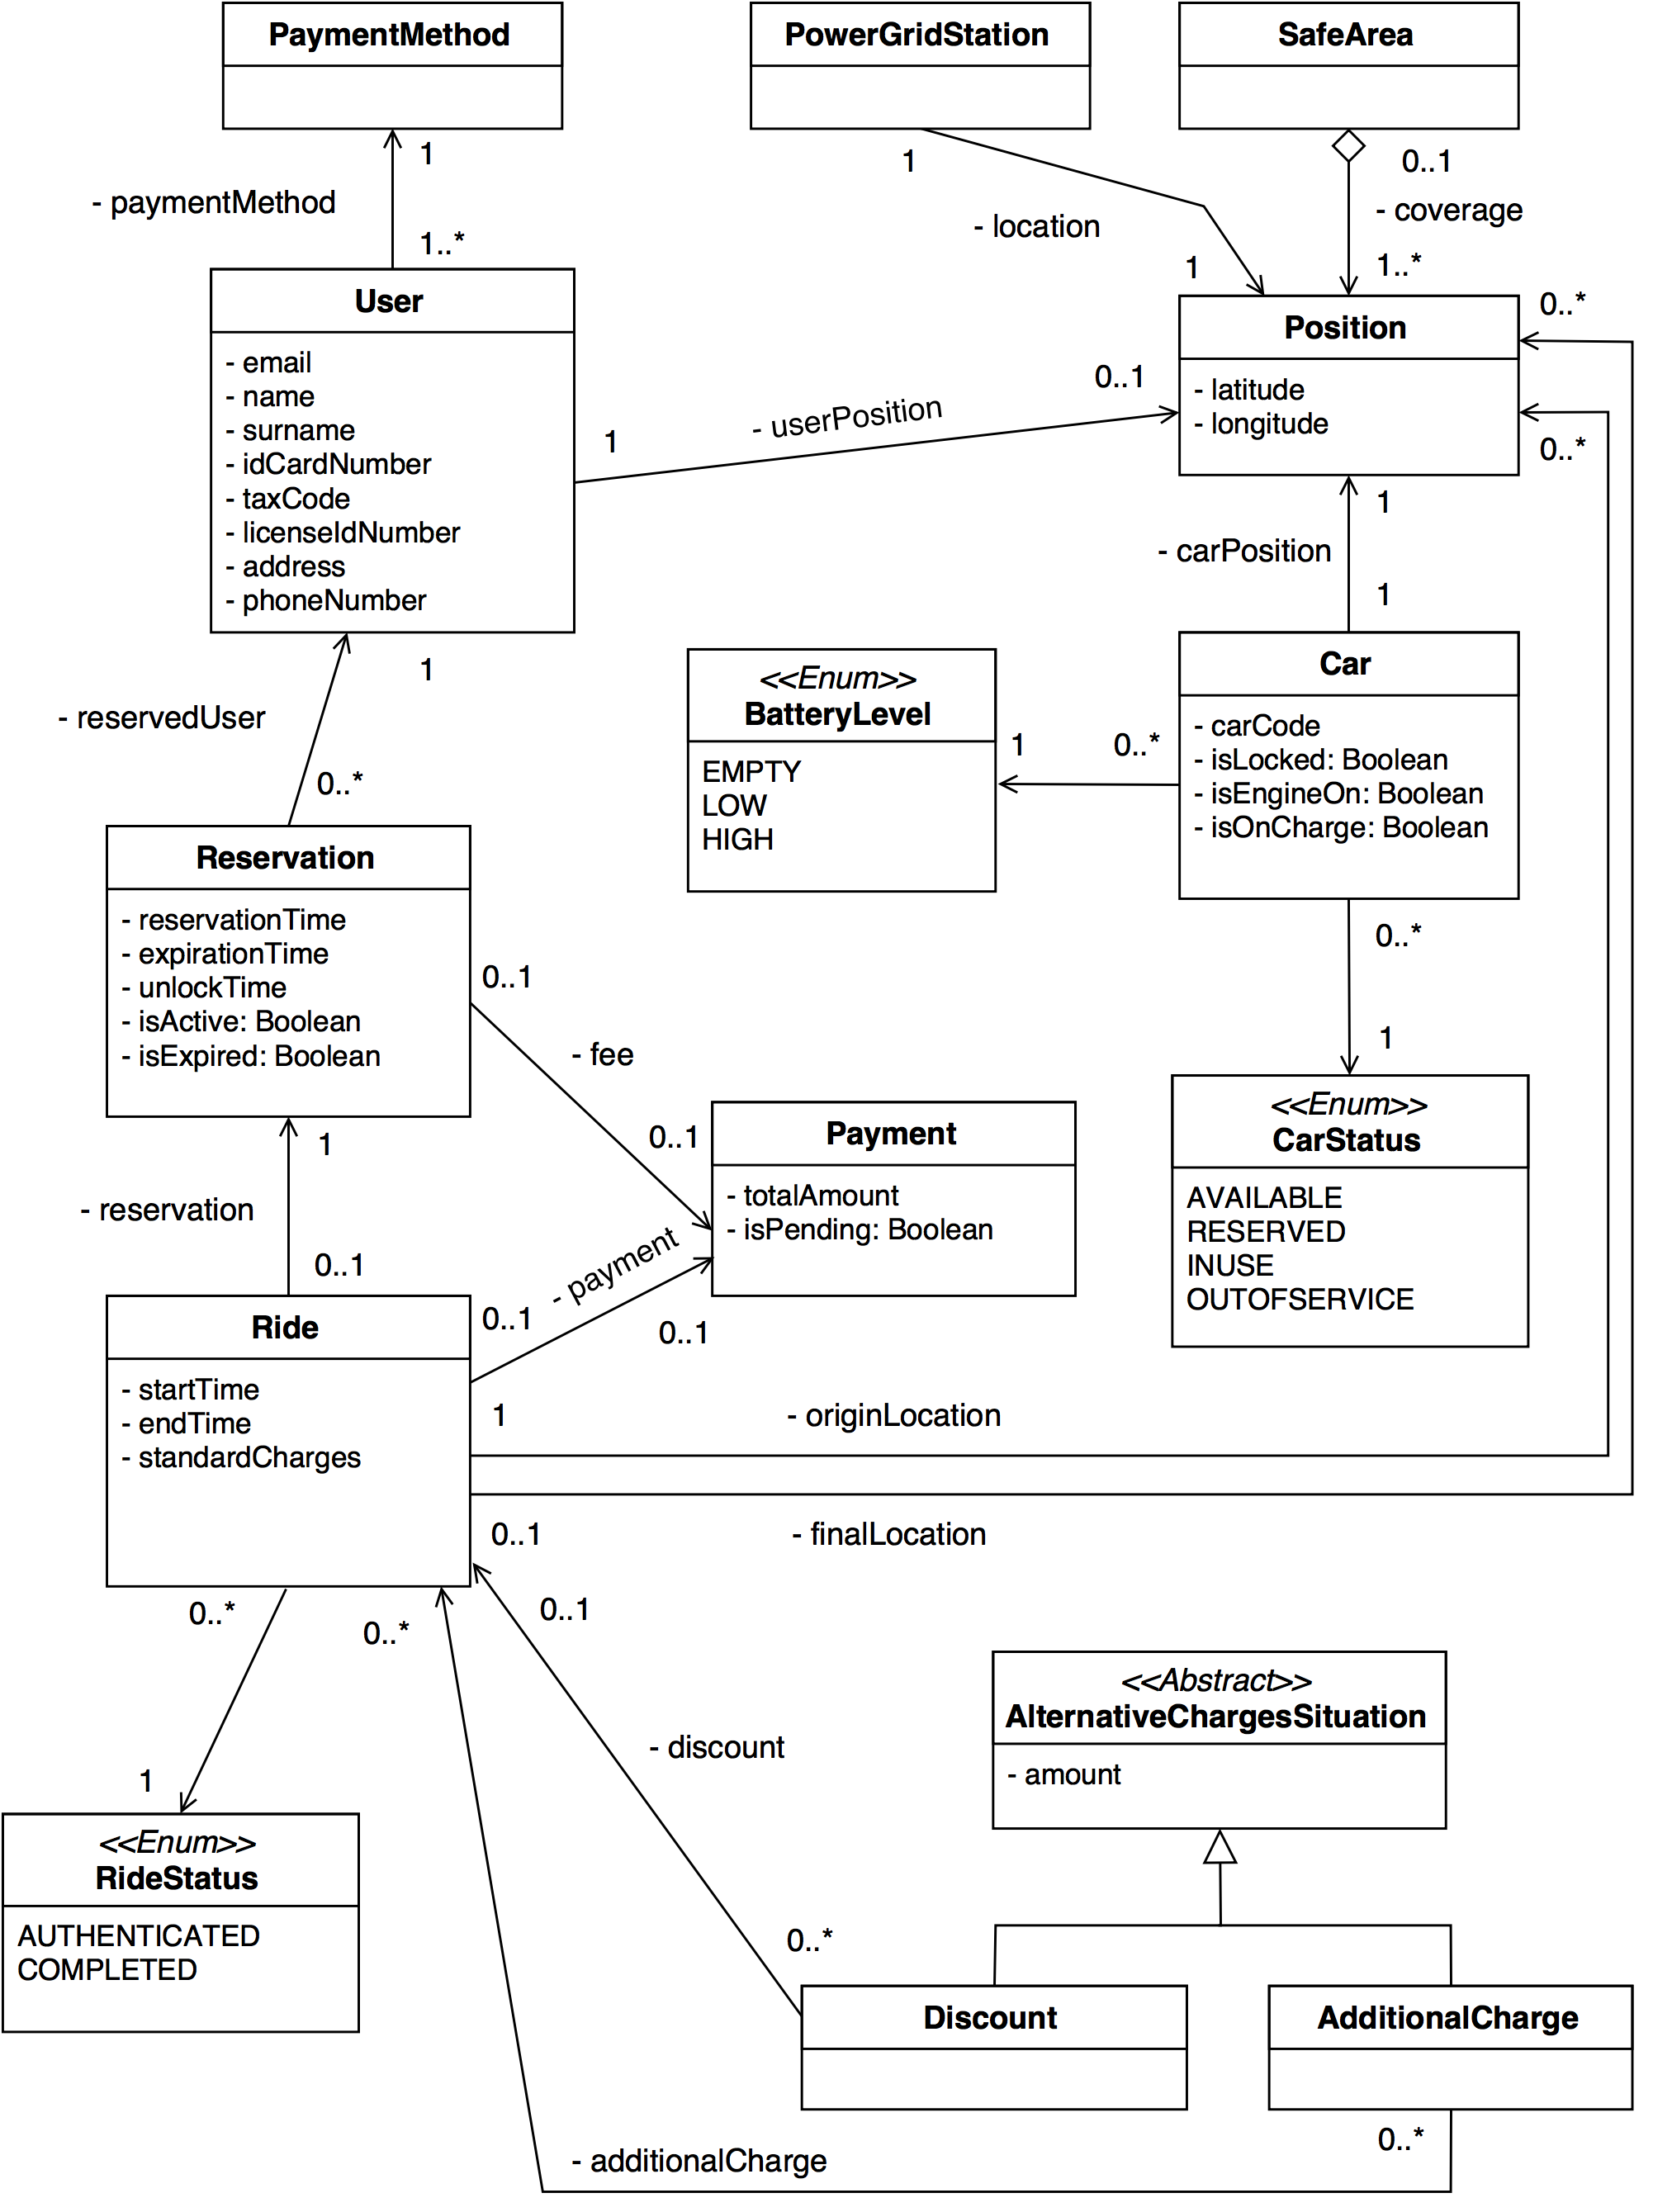
\includegraphics[width=\textwidth]{./pictures/class_diagram.png}
		\caption{Class diagram illustrating the structure of the system-to-be.}
		\label{class_diagram}
\end{center}
\end{figure}

% Settings for Alloy code listing.
\lstset{
    language=alloy,
    numbers=left,
    numberstyle=\tiny,
    stepnumber=2,
    tabsize=4,
    keywordstyle=\color{alloy-keyword}\bfseries,
    commentstyle=\color{alloy-comment},
    stringstyle=\color{alloy-string},
    basicstyle=\small\fontfamily{pcr}\selectfont, % Courier font family
}

% Includes the Alloy model file.
\lstinputlisting{./specific_requirements/alloy/alloy_pe.als}
